\begin{figure}
    \begin{small}
        \begin{center}
            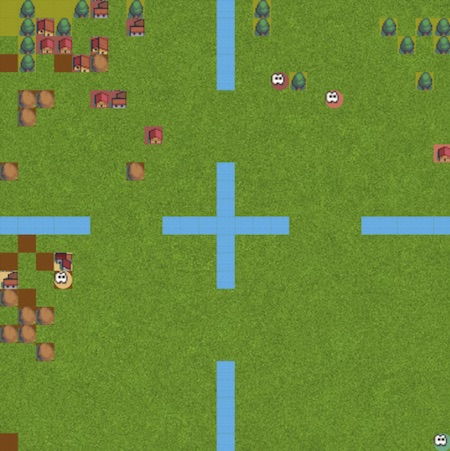
\includegraphics[width=0.4\textwidth]{figures/simulation_human_gui.jpg}
        \end{center}
        \caption{The Gather-and-Build game. Agents move around, collect resources (wood and stone) and build houses. Agents cannot move through each others' houses, or move through water. Agents can  trade resources.}
        \label{fig:simulation_human_gui}
    \end{small}
\end{figure}


\subsection{Environment Rules and Dynamics}
\label{sec:env_rules_and_dynamics}
\paragraph{Overview.}
We introduce the \textit{Gather-and-Build} game, a two-dimensional grid-world in which agents can move to collect resources, earn coins by using the resources of stone and wood to build houses, and trade with other agents to exchange resources for coins.
Stone and wood stochastically spawn on special resource regeneration tiles.
Agents can move around the environment to gather these resources from populated resource tiles that  remain empty after harvesting until some new resources spawn.

Agents can choose to use one unit of wood and one unit of stone to construct a house, and this places a house tile at the agent's current location and earns the agent some number of coins.
The number of coins earned per house depends on the {\em skill} of an agent, and skill is different across agents. In addition, agents start at different initial locations in the world.
These heterogeneities are the main driver of both economic inequality and specialization in our environment.


Agents can also trade resources, by submitting the number of coins they are willing to accept (an {\em ask}) or are willing to pay (a {\em bid}), respectively, to an open market, for each of wood and stone.
We provide a detailed description of the environment and its underlying dynamics in the appendix (Section~\ref{sec:details_of_environment}).

\paragraph{Labor and Skill.}
Over the course of an {\em episode} (a single play out of the environment), agents  accumulate labor cost, which reflects the amount of effort associated with the actions taken by the agent.
Each type of action (moving, gathering, trading, and building) is associated with a specific labor cost.
Each time an agent performs one of these actions, its accumulated labor is incremented by the action's associated labor cost.
As described below (Section \ref{sec:agent_utility}), agent rewards depend positively on accumulated coin and negatively on accumulated labor.
The labor costs associated with each action type are calibrated so that agents need to be strategic in how they choose to earn income, and all agents experience the same labor costs.

Following taxation theory, we allow agents in the environment to vary by  skill, which describes how much income an agent is able to earn per unit of labor.
We capture this by providing, separately for each agent, (1) a multiplier on the default number of coins earned from building a house, and (2) the probability of gaining bonus resources when harvesting.
The coin payoff for a house depends linearly on skill.
An agent receives a minimum of 10 coin per house built.

A {\em building skill} of 1 (the minimum value) means the agent earns this minimum payoff and a building skill of 2.5 means the agent receives 25 coin per house. The maximum skill value is 3.
An agent's {\em collection skill} is equal to the average number of resources it receives each time it steps on a populated stone or wood resource tile.
As an example, for an agent with a collection skill of 1.2, it will always receive at least 1 resource from stepping on a populated tile and there is a 20\% chance it will also receive a bonus unit of the collected resource.
The minimum collection skill is 1 and the maximum is 2, ranging from never receiving bonus resource units to always receiving them.

We conceptualize the coins that are generated when building a house as coming from a part of the wider economy that our simulation does not directly model. An agent's building skill--- the coin the agent receives from building ---reflects the value that this external market places on a particular agent's houses. The total quantity of coins generated by the simulated agents during an episode reflects the value created by their collective labor.

\paragraph{Environment Scenario.}
All experiments were carried out using the specific world map shown in Figure~\ref{fig:simulation_human_gui}, which has four quadrants,  mostly separated by water  from each other (this blocks movement), and with spatially clustered resources.
We focus on games with four agents, and apply a fixed set of building skills,
 chosen as the means of the quartiles of a clipped Pareto distribution with exponent $a=4$ and scale $m=1$.
Skills and starting locations are randomly assigned to agents.
These building skills correspond to payoffs of 11.3, 13.3, 16.5, and 22.2 coins per house.
In all  experiments, we used episodes of length $\eplen = 1000$ time steps.










